\documentclass{article}
\usepackage{graphicx} % Required for inserting images
\usepackage{amsmath, amsfonts, amssymb}
\usepackage[dvipsnames]{xcolor}
\usepackage{bbold}
\usepackage{float}
\usepackage{subcaption}
\usepackage{tikz}
\usepackage{logicpuzzle}
\usepackage{hyperref}
\usepackage{listings}
\usepackage{mdframed}
\usepackage[numbered,framed]{matlab-prettifier}
\lstset{
   style              = Matlab-editor,
   basicstyle         = \mlttfamily ,
   escapechar         = ",
   mlshowsectionrules = true,
}


% ========= Bibliography =========
% These lines load the `biblatex' package
% and read in the list of references from
% References.bib - take a look.
%
% To generate References.bib, I recommend https://www.mybib.com/
% rather than trying to write the .bib file yourself.
%
\usepackage{csquotes, biblatex}
\addbibresource{References.bib}
% ================================


\newtheorem{prop}{Proposition} % This defines a theorem-like environment. See https://www.overleaf.com/learn/latex/theorems_and_proofs
\newtheorem{lem}[prop]{Lemma}
\newtheorem{thm}[prop]{Theorem}
\newtheorem{cor}[prop]{Corollary}
\newtheorem{defn}[prop]{Definition}

\tikzset{thck/.style={black,line width=2pt},thn/.style={black,line width=0.5pt}}
\newcommand{\sudoku}[1]{%
    \begin{tikzpicture}
        \draw[thn] (0,0) grid (9,9);
        \draw[thck,line cap=rect] (0,0) grid[step=3] (9,9);
        
        \foreach \n [count=\i from 0] in {#1}
            {
            \pgfmathtruncatemacro{\x}{Mod(\i,9)}
            \pgfmathtruncatemacro{\y}{\i/9)}
            \node at (\x+0.5,9-\y-0.5) {\n};
            }
    \end{tikzpicture}
    }

\title{Quadratic Unconstrained Binary Optimization}
\author{Sam Muir }
\date{June 2024}

\begin{document}

\maketitle

\section{Introduction}

This project begins by covering how QUBO models can be constructed. Then we explore QUBO formulations of some well known combinatorial problems. We then apply these insights to the graph matching problem and the related quadratic assignment problem. Finally, we will discuss the feasibility of using 'quantum annealers' to solve QUBO problems. \\

\noindent This project will follow 'Continuous optimization methods for the graph isomorphism problem' by Stefan Klus and Patrick Gelß. This report will also contain MATLAB code showing QUBO implementations of each problem. The included code can be found at \href{https://github.com/muirsam/QUBO/}{https://github.com/muirsam/QUBO/}

\section{What are QUBO problems?}
\begin{defn}
A QUBO problem is an optimisation problem of form, 
\begin{align*}
    \min \: f(\mathbf{x}) = \mathbf{x}^T Q \mathbf{x} + d
\end{align*}
where \(\mathbf{x}\) is a vector of \(n\) binary variables, \(Q\) is a \(n \times n\) matrix and \(d\) is a constant.
\end{defn}

\noindent At first glance this definition seems quite limited. But using a few tricks we can convert many problems to this form.

\subsubsection{Simple Example}
\noindent Suppose we are given a set of four numbers \(\alpha = \{\alpha_1,\alpha_2, \dots \alpha_4\}\) and we need to find the two-element subset of \(\alpha\) with the largest sum. We can convert this into a QUBO problem as follows. \\

\noindent First define the binary decision vector \(\mathbf{x} = \begin{pmatrix}
	x_1 & x_2 & x_3 & x_n
	\end{pmatrix}^T\). 
Then the sum function can be written as \(\sum_{i=1}^4 \alpha_i x_i\). But since \(x_i\) is binary, \(x_i = x_i^2\) and so we can express the sum function as
\begin{align*}
\sum_{i=1}^4 \alpha_i x_i = \sum_{i=1}^4 \alpha_i x_i^2 = \mathbf{x}^T\begin{pmatrix}
	\alpha_1 & 0 & 0 & 0 \\
	0 & \alpha_2 & 0 & 0 \\
	0 & 0 & \alpha_3 & 0 \\ 
	0 & 0 & 0 & \alpha_4
\end{pmatrix}\mathbf{x}.
\end{align*} \\ 

\noindent If we chose to maximise this function the solution will not always be a two-element subset. Instead we can write the two-element constraint as \(\sum_{i=1}^n x_i = 2\). And since we want to punish functions which do not meet this condition, we create the penalty \(\bigg(\sum_{i=1}^4 x_i - 2\bigg)^2\) which can be expanded to get
\begin{align*}
	\bigg(\sum_{i=1}^4 x_i - 2\bigg)^2 &= \sum_{i=1}^4 x_i\sum_{j=1}^4 x_j - 4\sum_{i=1}^4 x_i + 4 \\
	&= \mathbf{x}^T \begin{pmatrix}
		1 & 1 & 1 & 1 \\
		1 & 1 & 1 & 1 \\
		1 & 1 & 1 & 1 \\
		1 & 1 & 1 & 1
	\end{pmatrix}\mathbf{x} - \mathbf{x}^T \begin{pmatrix}
		-4 & 0 & 0 & 0 \\
		0 & -4 & 0 & 0 \\
		0 & 0 & -4 & 0 \\
		0 & 0 & 0 & -4 
	\end{pmatrix}\mathbf{x} + 4 \\
	&= \mathbf{x}^T \begin{pmatrix}
		-3 & 1 & 1 & 1 \\
		1 & -3 & 1 & 1 \\
		1 & 1 & -3 & 1 \\
		1 & 1 & 1 & -3
	\end{pmatrix} \mathbf{x} + 4.
\end{align*}
If we multiply this penalty term by the weight \(\lambda = |\alpha_1| + |\alpha_2| + |\alpha_3| + |\alpha_4|\) we guarantee that the optimal solution will be a two-element subset. \\

\noindent Now we can write the problem as
\begin{align*}
	\max \: \mathbf{x}^T\begin{pmatrix}
		\alpha_1 & 0 & 0 & 0 \\
		0 & \alpha_2 & 0 & 0 \\
		0 & 0 & \alpha_3 & 0 \\ 
		0 & 0 & 0 & \alpha_4
	\end{pmatrix}\mathbf{x} - \mathbf{x}^T \lambda\begin{pmatrix}
	-3 & 1 & 1 & 1 \\
	1 & -3 & 1 & 1 \\
	1 & 1 & -3 & 1 \\
	1 & 1 & 1 & -3
	\end{pmatrix} \mathbf{x} - 4\lambda.
\end{align*}
where \(\lambda\) is the penalty weight. Cleaning this up and dropping the constant we get
\begin{align*}
	\min \: \mathbf{x}^T \begin{pmatrix}
		-\alpha_1 - 3\lambda & \lambda & \lambda & \lambda \\
		\lambda & -\alpha_2 - 3\lambda & \lambda & \lambda \\
		\lambda & \lambda & -\alpha_3 - 3\lambda & \lambda \\
		\lambda & \lambda & \lambda & -\alpha_4 - 3\lambda
	\end{pmatrix} \mathbf{x}.
\end{align*}

\newpage 

\noindent This can be implemented in code as
\begin{lstlisting}[language=MATLAB]
a = [a_1, a_2, a_3, a_4];
weight = sum(abs(a));
Q = diag(-a - 4*weight) + weight*ones(4);

solve(qubo(Q))
\end{lstlisting}
\noindent This is a simple example of creating a QUBO formulation of a problem. For more examples and a list of penalties corresponding to more complicated constraints, see \cite[p.~10]{tutorialQUBO} by Glover, Kochenberger and Du. Their tutorial is a great resource for understanding QUBO problems.\\

\noindent Also, using larger penalty weights will increase the runtime of most QUBO solving algorithms. So in many cases it is more efficient to estimate weight and check the solution for feasibility instead of using a massive weight.     

\subsection{Maximal Independent Set problem}

\noindent The maximal independent set of a graph is the largest subset of the vertex set such that no two vertices share an edge. 

\begin{figure}[H]
    \centering
    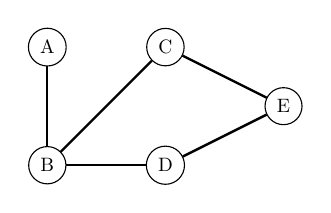
\begin{tikzpicture}
        \node[shape=circle,draw=black, scale=0.7] (A) at (0, 0) {A};
        \node[shape=circle,draw=black, scale=0.7] (B) at (0, -1.5) {B};
        \node[shape=circle,draw=black, scale=0.7] (C) at (1.5, 0) {C};
        \node[shape=circle,draw=black, scale=0.7] (D) at (1.5, -1.5) {D};
        \node[shape=circle,draw=black, scale=0.7] (E) at (3, -0.75) {E};
    
        \path [line width=0.3mm] (A) edge node[left] {} (B);
        
        \path [line width=0.3mm] (B) edge node[left] {} (C);
        \path [line width=0.3mm] (B) edge node[left] {} (D);

        \path [line width=0.3mm] (E) edge node[left] {} (C);
        \path [line width=0.3mm] (E) edge node[left] {} (D);
    \end{tikzpicture}
    \caption{This graph has maximal independent set \{A, C, D\}.}
\end{figure}

\noindent First we label the vertices of the graph \(x_1, \dots,  x_n\). If an edge connects vertices \(x_i\) and \(x_j\), we add the constraint \(x_i + x_j \leq 1\). \\

\noindent This constraint corresponds to the penalty \(2x_ix_j - x_i - x_j\) which is \(0\) when both vertices are included and \(-1\) otherwise. Then since \(x_i = x_i^2\) this penalty can be expressed in the form \(\mathbf{x}^T P_{edge}\mathbf{x}\). \\

\noindent Then we can sum these penalties to construct the matrix \(Q = \sum\limits_{edges} P_{edge}\). So the maximal independent set is the optimal solution of
\begin{align*}
    \min_{\mathbf{x} \in B(n)} \: \mathbf{x}^T Q \mathbf{x}.
\end{align*}
\noindent This can be implemented as
\begin{lstlisting}[language=MATLAB]
Q = zeros(n);
for i=1:n
    for j=1:n
        if A(i,j) == 1
            Q(i,i) = Q(i,i) - weight;
            Q(i,j) = Q(i,j) + weight;
        end
    end
end

solve(qubo(Q))
\end{lstlisting}

\subsection{Linear Assignment problem}

The linear assignment problem can be stated as:

Suppose we have \(n\) machines and \(n\) tasks which must be completed. We can assign any machine to do any task, but each task-machine pair has an associated cost. We want to allocate one machine to each task such that the sum of the costs is minimised. \\

\noindent If we let \(A\) be the matrix of machine-task costs then the problem can expressed as: 
\begin{align*}
    \min \: g(P) = \text{tr}(PA)
\end{align*}
where \(P\) is a permutation matrix which represents a task allocation. \\

\noindent We model this problem as a QUBO as follows: \\ 

\noindent First, let \(A = \begin{pmatrix}
    a_{11} & \hdots & a_{1n} \\
    \vdots & \ddots & \vdots \\
    a_{n1} & \hdots & a_{nn}
\end{pmatrix}\) and \(P = \begin{pmatrix}
    x_{1} & x_2 & \hdots & x_{n} \\
    x_{n + 1} & x_{n + 2} & \hdots & x_{2n} \\
    \vdots & \vdots & \ddots & \vdots \\
    x_{n(n-1)+1} & x_{n(n-1)+2} & \hdots & x_{n^2}
\end{pmatrix}\).
Then the function to be minimized is,
\begin{align*}
    \text{tr} (PA) &= \begin{pmatrix}
        x_1 \\
        \vdots \\
        x_n
    \end{pmatrix} \cdot \begin{pmatrix}
        a_{11}\\
        \vdots \\
        a_{n1}
    \end{pmatrix} + \begin{pmatrix}
        x_{n+1} \\
        \vdots \\
        x_{2n}
    \end{pmatrix} \cdot \begin{pmatrix}
        a_{12}\\
        \vdots \\
        a_{n2}
    \end{pmatrix} + \hdots + \begin{pmatrix}
        x_{n(n-1) + 1} \\
        \vdots \\
        x_{n^2}
    \end{pmatrix} \cdot \begin{pmatrix}
        a_{1n}\\
        \vdots \\
        a_{nn}
    \end{pmatrix} \\
    &= \sum_{i=1}^{n} \begin{pmatrix}
        x_{n(i-1) + 1} \\
        \vdots \\
        x_{ni}
    \end{pmatrix} \cdot \begin{pmatrix}
        a_{1i} \\
        \vdots \\
        a_{ni}
    \end{pmatrix} \\
    &= \sum_{i=1}^{n} \sum_{j=1}^{n} a_{ji}x_{n(i-1)+j}
\end{align*}
But since \(x_i\) is binary, \(x_i = x_i^2\), and so 
\begin{align*}
    \text{tr}(PA) &= \sum_{i=1}^{n} \sum_{j=1}^{n} a_{ji}x_{n(i-1)+j} \\
    &= \mathbf{x}^T \text{diag}(\text{vec}(A))\mathbf{x}.
\end{align*}\\
\noindent So we can now write the problem as 
\begin{align} \label{Ex:LinAss 1}
    \min g(\mathbf{x}) = \mathbf{x}^T \text{diag}(\text{vec}(A)) \mathbf{x}
\end{align}
where \(\mathbf{x} = \text{vec}(P^T)\) and \(P\) is a permutation matrix.\\

\noindent Now we need a penalty function which forces \(P\) to be a permutation matrix. To accomplish this we use the equation \(C\mathbf{x} = d\) given in \cite[p.~8]{klus2023continuous} where 
\begin{align}\label{mat:CD}
    C = \begin{pmatrix}
        \mathbb{1}_n^T & & \\
         & \ddots & \\ 
         & & \mathbb{1}_n^T \\
         e_1^T & \hdots & e_1^T \\
         \vdots & \ddots & \vdots \\
         e_n^T & \hdots & e_n^T
    \end{pmatrix} \in \mathbb{R}^{2n \times n^2}
\end{align}
and \(d = \mathbb{1}_{2n}\). \\

\noindent This equation is 0 if and only if \(P\) is doubly stochastic. But if \(P\) is doubly stochastic it is also a permutation matrix since each entry is binary. So this constraint forces \(P\) to be a permutation matrix.\\

\noindent We can transform the constraint \(C\mathbf{x} = d\) into the penalty \((C\mathbf{x} - d) \cdot (C\mathbf{x} - d)\). Adding this to (\ref{Ex:LinAss 1}) will favour solutions which are  permutation matrices.
Expanding this penalty we get,
\begin{align*}
    (C\mathbf{x} - d) \cdot (C\mathbf{x} - d) &= C\mathbf{x} \cdot C\mathbf{x} - 2d\cdot C\mathbf{x} + d \cdot d \\
    &= \mathbf{x}^T C^T C \mathbf{x} -2\mathbf{x}^T C^T d + d\cdot d
\end{align*}

\noindent Then since \(\mathbf{x}\) is binary \(x_i = x_i^2\) the linear term \(-2\mathbf{x}^T C^T d\) can be expressed as the quadratic term \(-2\mathbf{x}^T\text{diag}(C^Td)\mathbf{x}\). So the penalty term becomes
\begin{align}
    &\mathbf{x}^T C^T C \mathbf{x} -2\mathbf{x}^T\text{diag}(C^Td)\mathbf{x} + d\cdot d \nonumber \\
    = \: &\mathbf{x}^T(C^T C -2\text{diag}(C^Td))\mathbf{x} + d\cdot d. \label{penalty:CX}
\end{align}
And so we can rewrite problem (\ref{Ex:LinAss 1}) as 
\begin{align*}
    \min g(\mathbf{x}) = \mathbf{x}^T (\text{diag}(\text{vec}(A)) + \lambda C^T C - 2\lambda\text{diag}(C^T d))\mathbf{x} + \lambda d\cdot d
\end{align*}
where \(\lambda\) is the penalty weight. Then to get it in QUBO form we drop the consant to get
\begin{align*}
    \min g(\mathbf{x}) = \mathbf{x}^T Q \mathbf{x}
\end{align*}
where \(Q = \text{diag}(\text{vec}(A) - 2\lambda C^Td) + \lambda C^T C\).\\

\noindent This can be solved with the code:
\begin{lstlisting}[language=MATLAB]
Ct = transpose(C)
v = reshape(A, 1, [])
Q = diag(v - weight*2*Ct*d) + weight*Ct*C

x = solve(qubo(Q));
P = transpose(reshape(x.BestX, n, []))
\end{lstlisting}

\subsubsection{Example: Linear Assignment problem}

Consider the cost matrix, \begin{align*}
    A = \begin{pmatrix}
        7 & 9 & 1\\
        4 & 2 & 6\\
        7 & 8 & 7
    \end{pmatrix}
\end{align*}
where each column corresponds to a task and each row corresponds to the machine costs.

\noindent Using \(A\) and setting \(\lambda = 10\) we obtain the matrix
\begin{align*}
    Q = \begin{pmatrix}
        -13 & 10 & 10 & 10 & 0 & 0 & 10 & 0 & 0 \\
        10 & -16 & 10 & 0 & 10 & 0 & 0 & 10 & 0 \\
        10 & 10 & -13 & 0 & 0 & 10 & 0 & 0 & 10 \\
        10 & 0 & 0 & -11 & 10 & 10 & 10 & 0 & 0 \\
        0 & 10 & 0 & 10 & -18 & 10 & 0 & 10 & 0 \\
        0 & 0 & 10 & 10 & 10 & -12 & 0 & 0 & 10 \\
        10 & 0 & 0 & 10 & 0 & 0 & -19 & 10 & 10 \\
        0 & 10 & 0 & 0 & 10 & 0 & 10 & -14 & 10 \\
        0 & 0 & 10 & 0 & 0 & 10 & 10 & 10 & -13
    \end{pmatrix}
\end{align*}
Solving this gives \(X = \begin{pmatrix}
    0 & 0 & 1 & 0 & 1 & 0 & 1 & 0 & 0
\end{pmatrix}^T\)
and so we have \begin{align*}
    P = \begin{pmatrix}
        0 & 0 & 1 \\
        0 & 1 & 0 \\
        1 & 0 & 0
    \end{pmatrix}, \quad PA = \begin{pmatrix}
        7 & 8 & 7 \\
        4 & 2 & 6 \\
        7 & 9 & 1
    \end{pmatrix}
\end{align*}
which tells us that the minimum cost is \(\text{tr}(PA) = 10\).
\subsection{Sudoku}

In the game of Sudoku we are given a partially filled \(9 \times 9\) grid (81 squares) and the aim is to populate the remainder of the grid such that every column, row and box contains each of the numbers from 1 to 9. These boxes split the \(9 \times 9\) grid into 9 non-overlapping \(3 \times 3\) grids.\\

\hspace{92pt}\begin{lpsudoku}[scale=0.5]
\setrow{9}{6,5,{},{},{},7,9,{},3}
\setrow{8}{{},{},2,1,{},{},6,{},{}}
\setrow{7}{9,{},{},{},6,3,{},{},4}
\setrow{6}{1,2,9,{},{},{},{},{},{}}
\setrow{5}{3,{},4,9,{},8,1,{},{}}
\setrow{4}{{},{},{},3,{},{},4,7,9}
\setrow{3}{{},{},6,{},8,{},3,{},5}
\setrow{2}{7,4,{},5,{},{},{},{},1}
\setrow{1}{5,8,1,4,{},{},{},2,6}
\end{lpsudoku}\\
\\

\noindent We can formulate the Sudoku problem as follows. Following \cite[p.~1]{mücke2024sudoku} the vector \(\mathbf{x}\) will have 9 binary entries for each Sudoku square \(x_{i,j,k} = x_{81i + 9j + k}\). So each variable \(x_{i,j,k}\) is defined as
\begin{align*}
    x_{i,j,k} = \begin{cases}
        1 & \text{if row \(i\) column \(j\) has value \(k\)} \\
        0 & \text{otherwise.}
    \end{cases}
\end{align*}\\

\noindent The constraints of this problem are:
\begin{center}
\begin{tabular}{ |c|c| } 
 \hline
   & Constraint\\ 
 \hline
 a & Each column contains 1 to 9\\ 
 b & Each row contains 1 to 9\\
 c & Each box contains 1 to 9\\
 d & Every square must have a value\\
 \hline
\end{tabular}
\end{center}

\noindent Using \cite[p.~326]{ILPsudoku} the constraints above become
\begin{align*}
&\text{(a)} \quad \sum_{i=1}^9 x_{i,j,k} &&= 1\quad \forall j,k \in \{1 \dots 9\} \\
&\text{(b)} \quad \sum_{j=1}^9 x_{i,j,k} &&= 1\quad \forall i,k \in \{1 \dots 9\} \\
&\text{(c)} \quad \sum_{j=3q-2}^{3q} \sum_{i=3p-2}^{3p} x_{i,j,k} &&= 1\quad \forall k \in \{1 \dots 9\}, \forall p,q \in \{1 \dots 3\}\\
&\text{(d)} \quad \sum_{k=1}^9 x_{i,j,k} &&= 1\quad \forall i,j \in \{1 \dots 9\} \\
\end{align*}
where \(F\) is the set containing all triples corresponding to the indices of the filled squares. \\

\noindent We can transform these constraints into penalty functions by subtracting 1 and squaring them. Then to obtain a solution to these constraints we minimise the sum of these penalties. This means that the solved Sudoku will always be the optimal solution so we don't need to use penalty weights.\\

\noindent Consider constraint (a) for some fixed \(j\) and \(k\). Expanding the corresponding penalty gives us

\begin{align*}
    \bigg(\sum_{i=1}^9 x_{i,j,k} - 1\bigg)^2 &= \sum_{i=1}^9 x_{i,j,k}\sum_{p=1}^9 x_{p,j,k} -2\sum_{i=1}^9 x_{i,j,k} + 1  \\
    &= \sum_{i=1}^9\sum_{p=1}^9 x_{i,j,k}x_{p,j,k} -2\sum_{i=1}^9 x_{i,j,k}^2 + 1 \\
    &= \begin{pmatrix}
        x_{1,j,k} & \dots & x_{9,j,k}
    \end{pmatrix} (J_{9,9} - 2I) \begin{pmatrix}
        x_{1,j,k} \\
        \vdots \\
        x_{9,j,k}
    \end{pmatrix} + 1
\end{align*}
where \(J_{n, n}\) is the \(n \times n\) matrix of ones. \\

\noindent This we can replace \(\begin{pmatrix}
        x_{1,j,k} & \dots & x_{9,j,k}
    \end{pmatrix}^T\) with \(\mathbf{x}\) if we
    embed \(J_9 - 2I\) in a larger matrix with zeros everywhere but the rows and columns representing \(x_{1,j,k} \dots x_{9,j,k}\).\\

\noindent If we do this for every constraint and drop the constant we can add all 324 matrices to get a \(729 \times 729\) matrix \(U\)\footnote{This matrix is provided on the GitHub page under the name 'sudokuQ.mat' }.\\

\noindent Then we can take the squares which have already been filled and turn them into constraints. So the constraint \(x_{i,j,k} = 1\) becomes 
\begin{align*}
    (x_{i,j,k} - 1)^2 &= x_{i,j,k}^2 - 2x_{i,j,k} + 1 \\
    &= -x_{i,j,k}^2 + 1
\end{align*}
which can be interpreted as subtracting 1 from \((i,j,k)\)th element on the diagonal of \(U\). Doing this for every square which has been filled creates the matrix \(Q\).\\

\noindent Finally, solving the QUBO problem
\begin{align*}
    \min_{\mathbf{x} \in B(n)} \mathbf{x}^T Q \mathbf{x}
\end{align*}
will give us the \(\mathbf{x}\) which is a solution of the original Sudoku problem.\\

\noindent So the solution to the Sudoku is:

\hspace{92pt}\begin{lpsudoku}[scale=0.5]
\setrow{9}{6,5,8,2,4,7,9,1,3}
\setrow{8}{4,3,2,1,9,5,6,8,7}
\setrow{7}{9,1,7,8,6,3,2,5,4}
\setrow{6}{1,2,9,6,7,4,5,3,8}
\setrow{5}{3,7,4,9,6,8,1,6,2}
\setrow{4}{8,6,5,3,1,2,4,7,9}
\setrow{3}{2,9,6,7,8,1,3,4,5}
\setrow{2}{7,4,3,5,2,6,8,9,1}
\setrow{1}{5,8,1,4,3,9,7,2,6}
\end{lpsudoku}\\

\noindent The code for this QUBO implementation is on the GitHub under "sudoku.m".\\
 
\noindent Unfortunately, since \(Q\) is so large it is often not feasible to use this implementation to obtain solutions to Sudoku problems. A more efficient implementation of Sudoku is given by \cite{mücke2024sudoku}.

\section{Graph Isomorphism and Matching problems}
\subsection{The Graph Isomorphism problem}
Two graphs \(G_A\) and \(G_B\) are isomorphic if and only if there exists a bijection between the vertices of the graphs such that every edge which connects vertices in \(G_A\) corresponds to a edge connecting vertices in \(G_B\). \\
Essentially, an isomorphism means either graph can be redrawn and relabelled to be identical to the other. \\

\noindent So if the graphs have a different number of vertices or a different amount of edges, they cannot be isomorphic. You might think now that you can always find or rule out an isomorphism easily, but isomorphisms between graphs are not always obvious. For instance, can you tell if the graphs below are isomorphic?\\

\begin{figure}[H]
    \centering
    \hspace{48pt}
    \begin{subfigure}[h]{0.2\linewidth}
        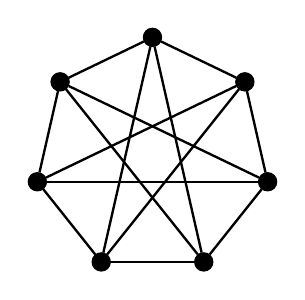
\begin{tikzpicture}
            \node[shape=circle,draw=black, fill=black, scale=0.7] (A) at (0, 1.5) {};
            \node[shape=circle,draw=black, fill=black, scale=0.7] (B) at (1.173, 0.935) {};
            \node[shape=circle,draw=black, fill=black, scale=0.7] (C) at (1.462, -0.334) {};
            \node[shape=circle,draw=black, fill=black, scale=0.7] (D) at (0.651, -1.352) {};
            \node[shape=circle,draw=black, fill=black, scale=0.7] (E) at (-0.651, -1.352) {};
            \node[shape=circle,draw=black, fill=black, scale=0.7] (F) at (-1.462, -0.334) {};
            \node[shape=circle,draw=black, fill=black, scale=0.7] (G) at (-1.173, 0.935) {};
        
            \path [line width=0.3mm] (A) edge node[left] {} (B);
            \path [line width=0.3mm] (A) edge node[left] {} (D);
            \path [line width=0.3mm] (A) edge node[left] {} (E);
            \path [line width=0.3mm] (A) edge node[left] {} (G);
        
            \path [line width=0.3mm] (B) edge node[left] {} (C);
            \path [line width=0.3mm] (B) edge node[left] {} (E);
            \path [line width=0.3mm] (B) edge node[left] {} (F);
        
            \path [line width=0.3mm] (C) edge node[left] {} (D);
            \path [line width=0.3mm] (C) edge node[left] {} (F);
            \path [line width=0.3mm] (C) edge node[left] {} (G);
        
            \path [line width=0.3mm] (D) edge node[left] {} (E);
            \path [line width=0.3mm] (D) edge node[left] {} (G);
        
            \path [line width=0.3mm] (E) edge node[left] {} (F);
        
            \path [line width=0.3mm] (F) edge node[left] {} (G);
        \end{tikzpicture}
    \end{subfigure}
    \hspace{40pt}
    \begin{subfigure}[h]{0.4\linewidth}
        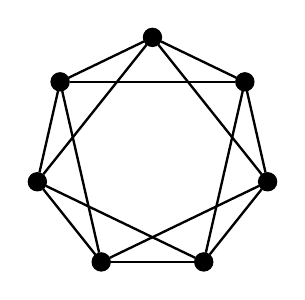
\begin{tikzpicture}
            \node[shape=circle,draw=black, fill=black, scale=0.7] (A) at (0, 1.5) {};
            \node[shape=circle,draw=black, fill=black, scale=0.7] (B) at (1.173, 0.935) {};
            \node[shape=circle,draw=black, fill=black, scale=0.7] (C) at (1.462, -0.334) {};
            \node[shape=circle,draw=black, fill=black, scale=0.7] (D) at (0.651, -1.352) {};
            \node[shape=circle,draw=black, fill=black, scale=0.7] (E) at (-0.651, -1.352) {};
            \node[shape=circle,draw=black, fill=black, scale=0.7] (F) at (-1.462, -0.334) {};
            \node[shape=circle,draw=black, fill=black, scale=0.7] (G) at (-1.173, 0.935) {};
        
            \path [line width=0.3mm] (A) edge node[left] {} (B);
            \path [line width=0.3mm] (A) edge node[left] {} (C);
        
            \path [line width=0.3mm] (B) edge node[left] {} (C);
            \path [line width=0.3mm] (B) edge node[left] {} (D);
        
            \path [line width=0.3mm] (C) edge node[left] {} (D);
            \path [line width=0.3mm] (C) edge node[left] {} (E);
        
            \path [line width=0.3mm] (D) edge node[left] {} (E);
            \path [line width=0.3mm] (D) edge node[left] {} (F);
        
            \path [line width=0.3mm] (E) edge node[left] {} (F);
            \path [line width=0.3mm] (E) edge node[left] {} (G);
        
            \path [line width=0.3mm] (F) edge node[left] {} (G);
            \path [line width=0.3mm] (F) edge node[left] {} (A);
        
            \path [line width=0.3mm] (G) edge node[left] {} (A);
            \path [line width=0.3mm] (G) edge node[left] {} (B);
        \end{tikzpicture}
    \end{subfigure}
    \caption{The graphs \(G_A\) (left) and \(G_B\) (right)}
    \label{fig:1}
\end{figure}

\noindent Now imagine trying to find an isomorphism between even larger graphs. Eventually, it is no longer possible to identify them by inspection and so we use algorithms to search for isomorphisms. \\

\noindent The graph isomorphism problem is the problem of determining whether any two graphs are isomorphic.\\

\noindent To interpret this as a QUBO problem we use some results from \autocite{klus2023continuous}. First,\\

\begin{lem}\label{lem:StochasticIso}
\cite[p.~6]{klus2023continuous} Suppose we have graphs \(G_A\) and \(G_B\) with adjacency matrices \(A\) and \(B\) respectively. The doubly stochastic relaxation of the graph isomorphism problem can be formulated as
\begin{equation*}
    c_D = \min_{X \in D(n)} ||XA - BX||^2_F
\end{equation*}
where \(D(n)\) is the set of doubly stochastic matrices and \(||\cdot||_F\) denotes the Frobenius norm.
\end{lem}

\begin{lem}\label{lem:qubo1}
    \cite[p.~8]{klus2023continuous} This optimisation problem can be written as \begin{align*}
    \min_{\substack{\mathbf{x} \in B(n) \\ C\mathbf{x} = d}} \mathbf{x}^T H\mathbf{x}
    \end{align*}
    with \(\mathbf{x} = \begin{bmatrix}
        X_1 \\
        \vdots \\
        X_n
    \end{bmatrix}\) where \(X_1, \dots X_n\) are the columns of \(X\), \(B(n)\) is the set of vectors with \(n\) binary entries, \(H = (A \otimes I_n - I_n \otimes B)^2\), and \(C\), \(d\) are defined by \ref{mat:CD}.
\end{lem}

\noindent Since we have shown in (\ref{penalty:CX}) that the constraint \(C\mathbf{x} = d\) corresponds to the penalty \(\mathbf{x}^T(C^T C - 2\text{diag}(C^T d))\mathbf{x}\), a QUBO formulation of this problem can be written as 
\begin{equation}\label{QUBO: graphIso1}
	\min_{x \in B(n)} \mathbf{x}^T Q \mathbf{x}
\end{equation}
where \(Q = H + \lambda C^T C - 2\lambda\text{diag}(C^T d)\) and \(\lambda\) is the penalty weight.\\

\noindent Alternatively, we can use Lemma 4.15 which states
\begin{lem}
	\cite[p.~13]{klus2023continuous} The optimisation problem can be written as \begin{align*}
		\min_{\substack{\mathbf{x} \in B(n) \\ C\mathbf{x} = d \\ H\mathbf{x}=0}} -\mathbf{x}^T\mathbf{x}
	\end{align*}
	where \(\mathbf{x}, C, d\) and \(H\) are defined as in (\ref{lem:qubo1})
\end{lem}

\noindent Since the constraint \(H\mathbf{x} = 0\) corresponds to the penalty \(H\mathbf{x} \cdot H\mathbf{x} =  \mathbf{x}^T H^T H  \mathbf{x}\) we can write a QUBO formulation of this problem as

\begin{equation}\label{QUBO: graphIso2}
	\min_{x \geq 0} \mathbf{x}^T Q \mathbf{x}
\end{equation}
where \(Q = -I_n + \lambda_1 C^T C - 2\lambda_1\text{diag}(C^T d) + \lambda_2 H^T H\) with penalty weights \(\lambda_1\) and \(\lambda_2\).\\

\noindent When we compare both QUBO implementations for the problem we find that generally implementation (\ref{QUBO: graphIso1}) is faster.

\subsubsection{Example: Graph Isomorphism problem}
Consider the graphs \(G_A\) and \(G_B\) from Figure \ref{fig:1}. \\

\noindent These graphs have the adjacency matrices
\begin{align*}
    A = \begin{pmatrix}
        0 & 1 & 0 & 1 & 1 & 0 & 1 \\
        1 & 0 & 1 & 0 & 1 & 1 & 0 \\
        0 & 1 & 0 & 1 & 0 & 1 & 1 \\
        1 & 0 & 1 & 0 & 1 & 0 & 1 \\
        1 & 1 & 0 & 1 & 0 & 1 & 0 \\
        0 & 1 & 1 & 0 & 1 & 0 & 1 \\
        1 & 0 & 1 & 1 & 0 & 1 & 0
    \end{pmatrix} \: \text{and }
    B = \begin{pmatrix}
        0 & 1 & 1 & 0 & 0 & 1 & 1 \\
        1 & 0 & 1 & 1 & 0 & 0 & 1 \\
        1 & 1 & 0 & 1 & 1 & 0 & 0 \\
        0 & 1 & 1 & 0 & 1 & 1 & 0 \\
        0 & 0 & 1 & 1 & 0 & 1 & 1 \\
        1 & 0 & 0 & 1 & 1 & 0 & 1 \\
        1 & 1 & 0 & 0 & 1 & 1 & 0
    \end{pmatrix}.
\end{align*}
when we enumerate their vertices clockwise. If we substitute \(A, B\) into (\ref{QUBO: graphIso1}), choose \(\lambda = 10\), and solve the QUBO problem we get
\begin{align*}
    X = \begin{pmatrix}
        0 & 1 & 0 & 0 & 0 & 0 & 0 \\
        0 & 0 & 0 & 0 & 0 & 1 & 0 \\
        0 & 0 & 1 & 0 & 0 & 0 & 0 \\
        0 & 0 & 0 & 0 & 0 & 0 & 1 \\
        0 & 0 & 0 & 1 & 0 & 0 & 0 \\
        1 & 0 & 0 & 0 & 0 & 0 & 0 \\
        0 & 0 & 0 & 0 & 1 & 0 & 0
    \end{pmatrix}
\end{align*}
which we find represents an isomorphism between \(G_A\) and \(G_B\).\\

\noindent Using this we find that the labelling  
\begin{figure}[H]
    \centering
    \hspace{48pt}
    \begin{subfigure}[h]{0.2\linewidth}
        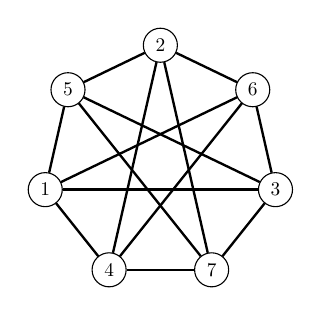
\begin{tikzpicture}
            \node[shape=circle,draw=black, scale=0.7] (A) at (0, 1.5) {2};
            \node[shape=circle,draw=black, scale=0.7] (B) at (1.173, 0.935) {6};
            \node[shape=circle,draw=black, scale=0.7] (C) at (1.462, -0.334) {3};
            \node[shape=circle,draw=black, scale=0.7] (D) at (0.651, -1.352) {7};
            \node[shape=circle,draw=black, scale=0.7] (E) at (-0.651, -1.352) {4};
            \node[shape=circle,draw=black, scale=0.7] (F) at (-1.462, -0.334) {1};
            \node[shape=circle,draw=black, scale=0.7] (G) at (-1.173, 0.935) {5};
        
            \path [line width=0.3mm] (A) edge node[left] {} (B);
            \path [line width=0.3mm] (A) edge node[left] {} (D);
            \path [line width=0.3mm] (A) edge node[left] {} (E);
            \path [line width=0.3mm] (A) edge node[left] {} (G);
        
            \path [line width=0.3mm] (B) edge node[left] {} (C);
            \path [line width=0.3mm] (B) edge node[left] {} (E);
            \path [line width=0.3mm] (B) edge node[left] {} (F);
        
            \path [line width=0.3mm] (C) edge node[left] {} (D);
            \path [line width=0.3mm] (C) edge node[left] {} (F);
            \path [line width=0.3mm] (C) edge node[left] {} (G);
        
            \path [line width=0.3mm] (D) edge node[left] {} (E);
            \path [line width=0.3mm] (D) edge node[left] {} (G);
        
            \path [line width=0.3mm] (E) edge node[left] {} (F);
        
            \path [line width=0.3mm] (F) edge node[left] {} (G);
        \end{tikzpicture}
    \end{subfigure}
    \hspace{40pt}
    \begin{subfigure}[h]{0.4\linewidth}
        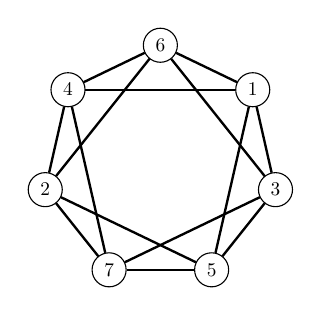
\begin{tikzpicture}
            \node[shape=circle,draw=black, scale=0.7] (A) at (0, 1.5) {6};
            \node[shape=circle,draw=black, scale=0.7] (B) at (1.173, 0.935) {1};
            \node[shape=circle,draw=black, scale=0.7] (C) at (1.462, -0.334) {3};
            \node[shape=circle,draw=black, scale=0.7] (D) at (0.651, -1.352) {5};
            \node[shape=circle,draw=black, scale=0.7] (E) at (-0.651, -1.352) {7};
            \node[shape=circle,draw=black, scale=0.7] (F) at (-1.462, -0.334) {2};
            \node[shape=circle,draw=black, scale=0.7] (G) at (-1.173, 0.935) {4};
    
            \path [line width=0.3mm] (A) edge node[left] {} (B);
            \path [line width=0.3mm] (A) edge node[left] {} (C);
        
            \path [line width=0.3mm] (B) edge node[left] {} (C);
            \path [line width=0.3mm] (B) edge node[left] {} (D);
        
            \path [line width=0.3mm] (C) edge node[left] {} (D);
            \path [line width=0.3mm] (C) edge node[left] {} (E);
        
            \path [line width=0.3mm] (D) edge node[left] {} (E);
            \path [line width=0.3mm] (D) edge node[left] {} (F);
        
            \path [line width=0.3mm] (E) edge node[left] {} (F);
            \path [line width=0.3mm] (E) edge node[left] {} (G);
        
            \path [line width=0.3mm] (F) edge node[left] {} (G);
            \path [line width=0.3mm] (F) edge node[left] {} (A);
        
            \path [line width=0.3mm] (G) edge node[left] {} (A);
            \path [line width=0.3mm] (G) edge node[left] {} (B);
        \end{tikzpicture}
    \end{subfigure}
\end{figure}
\noindent is an isomorphism.\\

\noindent The code for this implementation is
\begin{lstlisting}[language=MATLAB]
H = (kron(A, eye(n)) - kron(eye(n), B))^2;
Q = H + weight*(Ct*C - 2*diag(Ct*d));

x = solve(qubo(Q));
mat = reshape(x.BestX, [n,n]);
\end{lstlisting}

\subsection{Graph Matching and Quadratic Assignment problem}

\subsubsection{Graph Matching}

Given two weighted graphs \(G_A\) and \(G_B\), the graph matching problem is the problem of finding the bijection between the vertices of \(G_A\) and \(G_B\) which minimises the edge difference.\\

\noindent Essentially, the graph matching problem is a generalisation of the graph isomorphism problem to consider weighted matrices and non-isomorphic graphs.

\noindent The graph matching problem can be formulated as (\ref{lem:StochasticIso}) where \(A,B\) are weighted adjacency matrices. This means that it is equivalent to (\ref{lem:qubo1}) following the steps in \cite{klus2023continuous}.\\

\noindent So, the QUBO formulation of the graph matching problem is
\begin{equation*}
	\min_{\mathbf{x} \in B(n)} \mathbf{x}^T Q \mathbf{x}
\end{equation*}
where \(Q = (A \otimes I_n - I_n \otimes B)^2 + \lambda C^T C - 2\lambda\text{diag}(C^T d)\), \(\lambda\) is the penalty weight and \(C\), \(d\) are defined by \ref{mat:CD}.\\

\subsubsection{Example: Graph Matching}

Consider the graphs \(G_L\) and \(G_R\) on the left and right respectively. 
\begin{figure}[H]
    \centering
    \hspace{48pt}
    \begin{subfigure}[h]{0.2\linewidth}
        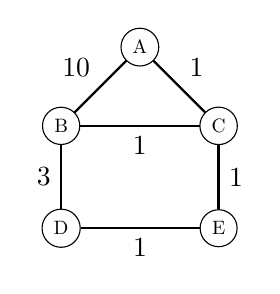
\begin{tikzpicture}
            \node[shape=circle,draw=black, scale=0.7] (A) at (0, 0) {A};
            \node[shape=circle,draw=black, scale=0.7] (B) at (-1, -1) {B};
            \node[shape=circle,draw=black, scale=0.7] (C) at (1, -1) {C};
            \node[shape=circle,draw=black, scale=0.7] (D) at (-1, -2.3) {D};
            \node[shape=circle,draw=black, scale=0.7] (E) at (1, -2.3) {E};
        
            \path[line width=0.3mm] (A) edge node[above left]{10} (B);
            \path [line width=0.3mm] (A) edge node[above right]{1} (C);

            \path [line width=0.3mm] (B) edge node[below]{1} (C);
            \path [line width=0.3mm] (B) edge node[left]{3} (D);

            \path [line width=0.3mm] (E) edge node[right]{1} (C);
            \path [line width=0.3mm] (E) edge node[below]{1} (D);
            
        \end{tikzpicture}
    \end{subfigure}
    \hspace{40pt}
    \begin{subfigure}[h]{0.4\linewidth}
        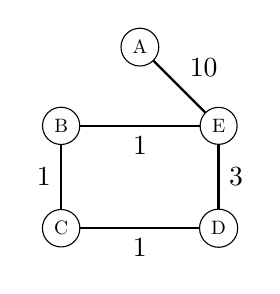
\begin{tikzpicture}
            \node[shape=circle,draw=black, scale=0.7] (A) at (0, 0) {A};
            \node[shape=circle,draw=black, scale=0.7] (B) at (-1, -1) {B};
            \node[shape=circle,draw=black, scale=0.7] (E) at (1, -1) {E};
            \node[shape=circle,draw=black, scale=0.7] (C) at (-1, -2.3) {C};
            \node[shape=circle,draw=black, scale=0.7] (D) at (1, -2.3) {D};
        
            \path[line width=0.3mm] (A) edge node[above right]{10} (E);

            \path[line width=0.3mm] (E) edge node[below]{1} (B);
            \path[line width=0.3mm] (E) edge node[right]{3} (D);

            \path[line width=0.3mm] (C) edge node[left]{1} (B);
            \path[line width=0.3mm] (C) edge node[below]{1} (D);
            
        \end{tikzpicture}
    \end{subfigure}
\end{figure}
\noindent These graphs have the adjacency matrices
\begin{align*}
    L = \begin{pmatrix}
        0 & 10 & 1 & 0 & 0 \\
        10 & 0 & 1 & 3 & 0 \\
        1 & 1 & 0 & 0 & 1 \\
        0 & 3 & 0 & 0 & 1 \\
        0 & 0 & 1 & 1 & 0
    \end{pmatrix}, \quad R = \begin{pmatrix}
        0 & 0 & 0 & 0 & 10 \\
        0 & 0 & 1 & 0 & 1 \\
        0 & 1 & 0 & 1 & 0 \\
        0 & 0 & 1 & 0 & 3 \\
        10 & 1 & 0 & 3 & 0
    \end{pmatrix}.
\end{align*}

\noindent Using these matrices, we find the solution of the graph matching problem is the permutation matrix
\begin{align*}
    X = \begin{pmatrix}
        1 & 0 & 0 & 0 & 0 \\
        0 & 0 & 1 & 0 & 0 \\
        0 & 0 & 0 & 0 & 1 \\
        0 & 0 & 0 & 1 & 0 \\
        0 & 1 & 0 & 0 & 0
    \end{pmatrix}
\end{align*}
which corresponds to the mapping from \(G_L\) to \(G_R\) which takes \(A \mapsto A, B \mapsto E, C \mapsto B, D \mapsto D\) and \(E \mapsto C\).


\subsubsection{Quadratic Assignment}

The quadratic assignment problem can be stated as:

Suppose we are given a set of \(n\) facilities and \(n\) locations, our job is to allocate each facility to a location such that we minimise the total cost. Each pair of facilities has a required flow and each pair of locations has a distance. The cost function is the sum of the flows multiplied by the distance for each facility-location pair.\\

\noindent Many real-world problems such to optimising building layouts, hospital transportation and scheduling can be expressed as quadratic assignment problems.\\

\noindent We can obtain a QUBO formulation of this as follows: \\
First let \(F\) and \(D\) be the flow and distance matrices where entries \(F_{ij}\) are the required flow between facilities \(i\) and \(j\) and \(D_{ij}\) is the distance between locations \(l_i\) and \(l_j\). Then the problem can be expressed as:
\begin{align*}
    \min_{X \in \mathcal{P}(n)} \: \text{tr}(FXD^TX^T).
\end{align*}

\noindent Using \cite[p.~3]{klus2023continuous} since \(X\) is a permutation matrix we have
\begin{align*}
    2\text{tr}(FXD^TX^T) = ||F||_F^2 + ||D||_F^2 - ||XF - DX||_F^2.
\end{align*}

\noindent Therefore minimising \(\text{tr}(FXD^TX^T)\) is equivalent to maximising \(||XF - DX||_F^2\) which is the negation of (\ref{lem:StochasticIso}) so the QUBO formulation of the quadratic assignment problem is the negation of (\ref{lem:qubo1})
\begin{equation*}
	\min_{\mathbf{x} \in B(n)} \mathbf{x}^T Q \mathbf{x}
\end{equation*}
where \(Q = -(A \otimes I_n - I_n \otimes B)^2 + \lambda C^T C -\lambda\text{diag}(C^T d)\), \(\lambda\) is the penalty weight and \(C\), \(d\) are defined by \ref{mat:CD}.\\

\section{Quantum Annealing}

One of the main reasons for constructing QUBO formulations of problems is that they are well-suited to being solved using quantum annealing. In this section we detail the connection between QUBO problems and quantum annealers. 

\subsection{Ising models}

First we need to modify our QUBO problems slightly to obtain the Ising models which quantum annealers are designed to solve.
Recall that the general form of a QUBO problem is
\begin{align*}
    \min_{x \in B(n)} \: f(\mathbf{x}) = \mathbf{x}^T Q \mathbf{x} + d.
\end{align*}

\noindent An Ising problem is an optimisation problem where the objective function is a quadratic function of multiple variables and each variable is either -1 or 1 (which are referred to as spins). We can convert a QUBO problem to an Ising formulation by applying the linear mapping \(s_i = 2x_i - 1\). The objective function values will then differ by 
\begin{align*}
    \mathbf{x}^T Q \mathbf{x} + d = \frac{1}{4} (\mathbf{s}^T + J_{1,n})Q(\mathbf{s} + J_{n,1}) + d 
\end{align*} 
where \(J_{i,j}\) is the \(i \times j\) matrix of ones.\\

\noindent The objective function of in the Ising formulation is referred to as the energy (so the optimal solution corresponds to the lowest energy). 

\subsection{Quantum Annealers}

\noindent This section is a abridged explanation of some of the ideas behind quantum annealing. For a more detailed explanation see \cite{tasseff2022emergingpotentialquantumannealing} and \cite{Yarkoni_2022}.\\

\noindent The idea behind quantum annealing is as follows. First we create an Ising formulation of the target problem, and label the objective we are looking to minimise the 'final Hamiltonian'.

\noindent Then we prepare a quantum system in its ground state of an easy to solve function known as the 'initial Hamiltonian'. If we slowly interpolate between the initial and the final Hamiltonian, the Adiabatic theorem \cite{Yarkoni_2022} ensures that the quantum system remains in the ground state. At the end, this ground state will correspond to the optimal solution of the target problem.\\

\noindent This process is analogous the the technique of annealing metal where a metal is heated above its recrystallization temperature and slowly cooled to increase strength and reduce stress.

\noindent A great explanation of the physical mechanism underlying quantum annealing is given in \cite{quantumAnnealingDWave} by D-Wave Systems who are the leading providers of quantum annealers. \\

\subsection{Limitations}

As shown in \cite{tasseff2022emergingpotentialquantumannealing}, there is some evidence that quantum annealers can provide a performance advantage for certain problems. But this advantage has not been conclusively demonstrated over the fastest classical algorithms.\\

\noindent The largest commercial quantum annealer is D-Wave System's 5000 qubit Advantage system. This system allows each 15 couplers per qubit effectively means each column in the QUBO matrix must have less than 16 entries. This could mean that some QUBO formulations are infeasible to solve using the Advantage system.\\

\noindent Unfortunately the MATLAB code provided is not yet compatible with D-Wave Systems quantum annealers. But it is compatible with IBM's remote Qiskit service. 

\section{Conclusion}



Any binary integer programming problem can be formulated as a QUBO problem. 

\nocite{*}
\printbibliography % This command prints the cited references.

\end{document}
